%% main.tex
%% Manuscript prepared for IEEE Transactions on Geoscience and Remote Sensing (TGRS).
%% Compile: pdflatex main && bibtex main && pdflatex main && pdflatex main
%% (or: latexmk -pdf main.tex). All figures are in ./figures; diagrams are drawn in TikZ.
\documentclass[journal]{IEEEtran}

\usepackage[T1]{fontenc}
\usepackage{cite}
\usepackage{amsmath,amssymb}
\usepackage{graphicx}
\usepackage{booktabs}
\usepackage{multirow}
\usepackage{array}
\usepackage{xcolor}
\usepackage{url}
\usepackage{xurl}
\usepackage{placeins}
\usepackage[ruled,vlined,linesnumbered]{algorithm2e}
\usepackage{tikz}
\usetikzlibrary{arrows.meta,positioning,fit,backgrounds,calc,shapes.geometric}
\usepackage[hidelinks]{hyperref}

\graphicspath{{figures/}}

\newcommand{\cdr}{CDR-PINO}
\newcommand{\auc}{ROC-AUC}

\hyphenation{op-tical net-works semi-conduc-tor sus-cep-ti-bil-i-ty}

\begin{document}

\title{Does a Governing Equation Help? A Controlled Evaluation of a Convection-Diffusion-Reaction Physics-Informed Neural Operator for Forest Fire Susceptibility Mapping in India}

\author{Author~Name,~\IEEEmembership{Student Member,~IEEE,}
        Second~Author,
        and~Third~Author%
\thanks{Manuscript received Month DD, 2026. (Corresponding author: Author Name.)}%
\thanks{A. Name is with the Department of ..., University ..., City, India (e-mail: author@example.com).}%
\thanks{The code, result files and per-cell predictions used in this study are available in the project repositories listed in the Data Availability section.}}

\markboth{IEEE Transactions on Geoscience and Remote Sensing}%
{Author \MakeLowercase{\textit{et al.}}: Controlled Evaluation of a CDR Physics-Informed Neural Operator for Fire Susceptibility}

\maketitle

\begin{abstract}
Embedding a governing equation in a learning model is widely expected to improve environmental prediction, particularly when test conditions differ from training conditions. For forest fire susceptibility this expectation has not been examined under controlled conditions. We built a physics-informed Fourier neural operator whose latent field obeys a convection-diffusion-reaction (CDR) equation, with diffusion, advection and reaction coefficients driven by vegetation and moisture, terrain, and access covariates, and trained it on monthly MODIS fire detections over India from 2000 to 2022. The model was compared with three controls: the same network trained without the equation, classical models fitted on exactly the same cells, splits and covariates, and baselines that use no covariates at all. The comparison covered random, spatial block, held-out region and held-out year evaluation, three random seeds and paired significance tests. No physics configuration improved on the network without physics. On the random split the full CDR model reached a \auc{} of 0.939 against 0.945 without the equation (DeLong $p<0.02$ for every seed), and on spatial and regional hold-out the differences could not be distinguished from zero. On identical 12 km cells and covariates a random forest scored 0.980, 0.974 and 0.959 on the random, spatial and regional tracks, compared with 0.939, 0.719 and 0.570 for the operator. For held-out years the operator (0.893) scored below a climatological fire frequency baseline (0.908) and a seasonal frequency baseline (0.930). Diagnostics of the trained field showed a nearly static solution whose equation residual was 74 to 616 times its own rate of change. The analysis rests on a rebuilt national pipeline with 541\,545 forest fire points, 55 predictors on a 1/120 degree grid, a corrected fire label and seasonal trend statistics, in which a random forest reaches 0.975 over all pixels and 0.897 over forest pixels. The accuracy differences observed in this problem are explained by the model family and the predictor set, not by the physics.
\end{abstract}

\begin{IEEEkeywords}
Forest fire, susceptibility mapping, physics-informed machine learning, Fourier neural operator, convection-diffusion-reaction, spatial cross-validation, MODIS, India.
\end{IEEEkeywords}

\IEEEpeerreviewmaketitle

%% =====================================================================
\section{Introduction}
%% =====================================================================

\IEEEPARstart{F}{orest} fires are a recurring hazard across India, and roughly a third of the national forest area is classed as fire prone in official assessments cited by recent work \cite{biswas2025}. Maps that rank locations by their long-term likelihood of burning are used to plan patrols, fuel treatment and early warning. The most recent national map was produced by Biswas \emph{et al.} \cite{biswas2025}, who trained a maximum entropy (MaxEnt) model on fifteen static predictors at 0.25 degree resolution and reported a test area under the receiver operating characteristic curve of 0.879.

Regional studies in India use a wide range of learners. Examples include analytic hierarchy weighting combined with tree ensembles in Goa \cite{uthappa2025}, a six-model ensemble for the Western Ghats \cite{kandanaveenbabu2023}, MaxEnt in Tamil Nadu \cite{meraj2025}, boosted and bagged trees in Odisha \cite{guria2025}, six learners in Mizoram \cite{gupta2025}, stacked ensembles in the northeast \cite{sarkar2024}, explainable ensembles in the Western Himalaya \cite{hang2024} and fuzzy weighting in Jammu and Kashmir \cite{malik2025}. Studies elsewhere follow the same pattern, with convolutional networks in Yunnan \cite{zhang2019}, random forests and neural networks in Turkey \cite{kantarcioglu2023,iban2024}, gradient boosting in New South Wales and Greece \cite{zakari2025,symeonidis2025}, evidential learning in Iran \cite{gholamnia2026} and driver analysis in Portugal \cite{santananeto2025}. Nearly all of this work treats susceptibility as a static classification of locations and reports a single random split, although spatially blocked validation is recommended whenever the data are spatially autocorrelated \cite{roberts2017}.

Physics-informed neural networks add the residual of a differential equation to the training loss \cite{raissi2019}, and neural operators learn mappings between whole fields on a grid \cite{li2023pino}. Fourier neural operators have been applied to climate downscaling \cite{jiang2023}, hydrological ensembles \cite{sun2024} and global weather forecasting \cite{kurth2023}. The arguments usually made for physics-informed learning are better behaviour when data are scarce or shifted, physically consistent outputs and mechanistic interpretability \cite{karniadakis2021}, and process guidance has been shown to help lake temperature prediction when training data are thinned \cite{read2019}. In the fire domain, physics-informed methods have so far addressed fire spread and data assimilation for individual events \cite{vogiatzoglou2025,dabrowski2023}, not susceptibility over a country.

The open question is therefore not whether a physics-informed susceptibility model can be built, but whether the equation contributes anything once other factors are held fixed. These factors include the capacity of the network, the choice of predictors, the grid and evaluation population, and the structure of the test split. Separating them requires controls that are rarely reported together: the same network without the equation, classical learners given identical inputs, and baselines that use no covariates. We address four research questions.
\begin{itemize}
\item \textbf{RQ1.} Do diffusion, advection and reaction terms improve held-out discrimination relative to the same network trained without them, under random, spatial, regional and temporal splits?
\item \textbf{RQ2.} How does the operator compare with classical models trained on the same cells, partitions and covariates?
\item \textbf{RQ3.} For held-out years, does the operator outperform baselines that ignore covariates?
\item \textbf{RQ4.} Does the trained operator behave as a solution of its own equation?
\end{itemize}

The contributions of this paper are as follows.
\begin{enumerate}
\item A controlled test of a physics-informed operator for fire susceptibility: four physics configurations, four evaluation tracks and three seeds, with paired tests, same-cell classical comparisons and persistence baselines. The answer to RQ1 to RQ3 is negative, and a paired decomposition locates where the accuracy differences actually arise.
\item A physical consistency diagnostic based on term magnitudes and the equation residual of the trained field, which shows that a physics-regularised model can score well while its field neither evolves in time nor satisfies the equation (RQ4).
\item A reproducible national pipeline for India in which every statistic was recalculated from raw data. It corrects a half-pixel misregistration of fire points, replaces degenerate anomaly predictors with climatological levels, replaces Mann-Kendall tests on seasonal series with the Seasonal Kendall test, restricts spatial autocorrelation to cells inside the country and uses land cover from before the label period. Forest pixels are evaluated as the primary population.
\item A reimplementation of the reference MaxEnt protocol on the same data, which places the reference result in context and states which pixel-level scores can and cannot be compared with it.
\end{enumerate}

The paper is organised as follows. Section~\ref{sec:data} describes the study area, data and predictors. Section~\ref{sec:methods} presents the classical models, the operator and the evaluation design. Section~\ref{sec:results} reports the results, Section~\ref{sec:discussion} interprets them and Section~\ref{sec:conclusion} concludes.

%% =====================================================================
\section{Study Area and Data}
\label{sec:data}
%% =====================================================================

\subsection{Domain, Period and Grid}
The study area is India, delimited by a dissolved state boundary polygon reprojected to geographic coordinates (EPSG:4326). The study period runs from 1 November 2000 to 15 December 2022 (266 months), bounded by the availability of annual ESA CCI and C3S land cover maps. All raster products are aligned to a common grid of $3641\times3504$ cells with a spacing of 1/120 degree (about 0.93 km). The India mask contains 4\,184\,671 cells, of which 4\,160\,768 have valid vegetation data and form the analysis population. Cells with a 2001 forest fraction above zero (1\,197\,538 cells) form the forest population.

\subsection{Fire Observations and Label}
Active fire detections were taken from the MODIS Collection 6.1 archive \cite{giglio2016}. Clipping to a bounding box, clipping to the India polygon, removing duplicates by location and date, and keeping only detections that fall on a forest class of the same year's land cover map (thirteen forest codes) reduced 2\,804\,373 records to 541\,545 forest fire points. Detections with confidence below 30 (4.29\%) and non-vegetation type codes (0.21\%) were retained, because excluding either group changed \auc{} by less than 0.001. Annual counts agree with those implied by the published shares of \cite{biswas2025} to within 0.5\% to 2.4\% ($r=0.99996$, 2001 to 2020). Forest cover inside the Indian boundary ranges from 18.3\% to 19.3\% over the period.

A cell is labelled positive if it contains at least one forest fire point during the study period. Each point is assigned to the cell that contains it,
\begin{equation}
c=\left\lfloor \frac{\lambda-x_0}{\Delta x}\right\rfloor,\qquad
r=\left\lfloor \frac{\varphi-y_0}{\Delta y}\right\rfloor ,
\label{eq:rasterise}
\end{equation}
where $(x_0,y_0)$ is the outer corner of the grid, $(\lambda,\varphi)$ are the point coordinates and $\Delta y<0$. The label has 268\,411 positive cells, a prevalence of 6.45\% over all cells and 22.4\% over forest cells. Rounding instead of flooring in (\ref{eq:rasterise}) measures from the cell edge rather than the cell centre and moves 74.9\% of points into a neighbouring cell. Correcting it raises random forest \auc{} by 0.006 over all pixels and 0.011 over forest pixels.

\subsection{Predictors}
The 55 predictors are summarised in Table~\ref{tab:predictors}. They cover all fifteen variable groups of \cite{biswas2025}. Climate and land surface temperature enter as 2001 to 2020 climatological levels together with a Seasonal Kendall trend statistic. Land cover fractions are taken from the 2001 map so that they precede almost the whole label period. Three design points deserve comment. First, a time mean of anomalies computed against a 2001 to 2020 baseline equals the residue of the 26 months outside the baseline, so it carries almost no spatial information: the spatial standard deviation of each climatological level is 40 to 431 times that of its anomaly mean. Second, five variable groups come from products that differ from those of the reference study (MOD11A2 for land surface temperature, MOD13A3 for vegetation, and FLDAS for precipitation, soil moisture and net longwave radiation). Third, distances were validated against exact geodesic distances at 3000 random locations, with root mean square errors of 0.31, 0.65 and 0.32 km for roads, railways and waterways.

\begin{table}[!t]
\caption{Predictor Set Used by the Classical Models (55 Features)}
\label{tab:predictors}
\centering
\footnotesize
\renewcommand{\arraystretch}{1.15}
\begin{tabular}{@{}p{1.45cm}p{1.9cm}p{4.3cm}@{}}
\toprule
Group (count) & Source & Features \\
\midrule
Vegetation (6) & MOD13A3.061, 1 km, monthly & QA-masked mean NDVI; climatological June NDVI; Seasonal Kendall $\tau$; seasonal Sen slope; CVSI at lag $k^\ast=8$; LISA cluster class \\
Surface temp. (6) & MOD11A2.061, 1 km, 8-day & Climatological level and Seasonal Kendall $\tau$ of day LST, night LST and diurnal range \\
Climate (14) & FLDAS Noah, 0.1$^\circ$, monthly & Level and Seasonal Kendall $\tau$ of air temperature, specific and relative humidity, wind, precipitation, net longwave radiation and soil moisture \\
Terrain (4) & SRTMGL3, 90 m & Elevation; Horn slope \cite{horn1981}; sine and cosine of aspect \\
Access (3) & OpenStreetMap 2022 & Distance to roads, railways and waterways \\
Land cover (22) & ESA CCI/C3S 2001 & 21 class fractions and forest fraction \\
\bottomrule
\end{tabular}
\end{table}

%% =====================================================================
\section{Methods}
\label{sec:methods}
%% =====================================================================

Fig.~\ref{fig:workflow} gives an overview of the workflow, from the raw products to the two model branches and the evaluation stage.

\begin{figure*}[!t]
\centering
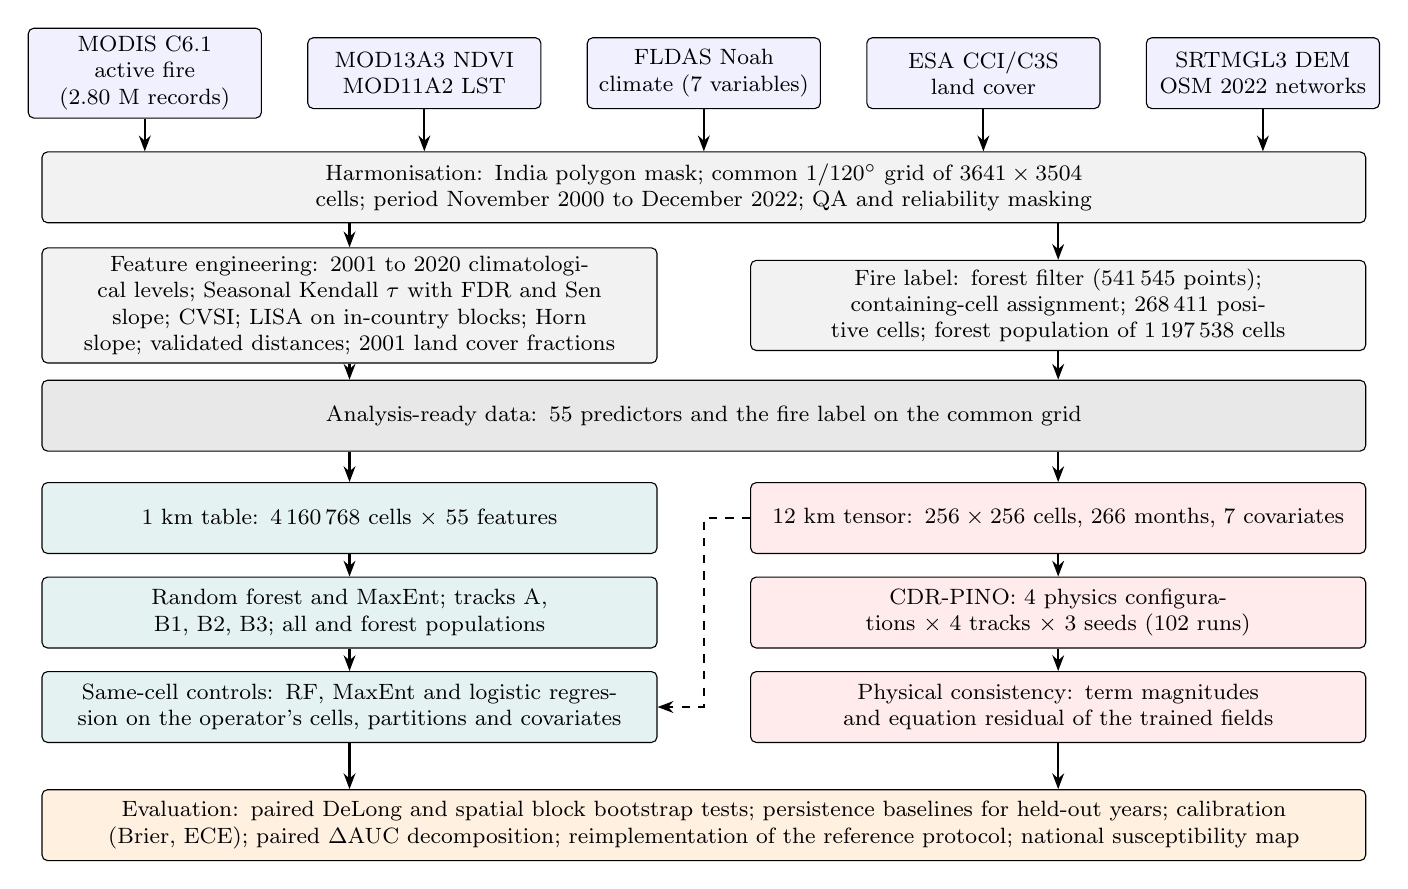
\begin{tikzpicture}[
  font=\footnotesize,
  box/.style={draw, rounded corners=2pt, align=center, minimum height=0.9cm, fill=white, inner sep=3pt},
  src/.style={box, fill=blue!6, text width=2.75cm},
  proc/.style={box, fill=gray!10},
  cls/.style={box, fill=teal!10, text width=7.6cm},
  phy/.style={box, fill=red!8, text width=7.6cm},
  eva/.style={box, fill=orange!12, text width=16.6cm},
  arr/.style={-{Stealth[length=2mm]}, thick}]
% sources (row 1)
\node[src] (fire) at (0.0,0) {MODIS C6.1 active fire\\(2.80 M records)};
\node[src] (veg)  at (3.55,0) {MOD13A3 NDVI\\MOD11A2 LST};
\node[src] (clim) at (7.10,0) {FLDAS Noah\\climate (7 variables)};
\node[src] (lc)   at (10.65,0) {ESA CCI/C3S\\land cover};
\node[src] (terr) at (14.20,0) {SRTMGL3 DEM\\OSM 2022 networks};
% harmonisation (row 2)
\node[proc, text width=16.6cm] (harm) at (7.10,-1.45) {Harmonisation: India polygon mask; common 1/120$^\circ$ grid of \mbox{$3641\times3504$} cells; period November 2000 to December 2022; QA and reliability masking};
% features and label (row 3)
\node[proc, text width=7.6cm] (feat) at (2.60,-2.95) {Feature engineering: 2001 to 2020 climatological levels; Seasonal Kendall $\tau$ with FDR and Sen slope; CVSI; LISA on in-country blocks; Horn slope; validated distances; 2001 land cover fractions};
\node[proc, text width=7.6cm] (lab)  at (11.60,-2.95) {Fire label: forest filter (541\,545 points); containing-cell assignment; 268\,411 positive cells; forest population of 1\,197\,538 cells};
% merged analysis-ready data (row 4)
\node[proc, text width=16.6cm, fill=gray!18] (ready) at (7.10,-4.35) {Analysis-ready data: 55 predictors and the fire label on the common grid};
% branches (rows 5 to 7)
\node[cls] (tab)    at (2.60,-5.65) {1 km table: 4\,160\,768 cells $\times$ 55 features};
\node[phy] (ten)    at (11.60,-5.65) {12 km tensor: $256\times256$ cells, 266 months, 7 covariates};
\node[cls] (clsm)   at (2.60,-6.85) {Random forest and MaxEnt; tracks A, B1, B2, B3; all and forest populations};
\node[phy] (cdrm)   at (11.60,-6.85) {\cdr{}: 4 physics configurations $\times$ 4 tracks $\times$ 3 seeds (102 runs)};
\node[cls] (bridge) at (2.60,-8.05) {Same-cell controls: RF, MaxEnt and logistic regression on the operator's cells, partitions and covariates};
\node[phy] (diag)   at (11.60,-8.05) {Physical consistency: term magnitudes and equation residual of the trained fields};
% evaluation (row 8)
\node[eva] (eval) at (7.10,-9.55) {Evaluation: paired DeLong and spatial block bootstrap tests; persistence baselines for held-out years; calibration (Brier, ECE); paired $\Delta$AUC decomposition; reimplementation of the reference protocol; national susceptibility map};
% arrows
\foreach \s in {fire,veg,clim,lc,terr} \draw[arr] (\s.south) -- (\s.south |- harm.north);
\draw[arr] (feat.north |- harm.south) -- (feat.north);
\draw[arr] (lab.north |- harm.south) -- (lab.north);
\draw[arr] (feat.south) -- (feat.south |- ready.north);
\draw[arr] (lab.south) -- (lab.south |- ready.north);
\draw[arr] (tab.north |- ready.south) -- (tab.north);
\draw[arr] (ten.north |- ready.south) -- (ten.north);
\draw[arr] (tab) -- (clsm);
\draw[arr] (ten) -- (cdrm);
\draw[arr] (clsm) -- (bridge);
\draw[arr] (cdrm) -- (diag);
\draw[arr, dashed] (ten.west) -- (7.10,-5.65) |- (bridge.east);
\draw[arr] (bridge.south) -- (bridge.south |- eval.north);
\draw[arr] (diag.south) -- (diag.south |- eval.north);
\end{tikzpicture}
\caption{Workflow of the study. Blue boxes are raw data products, grey boxes are shared preprocessing, green boxes form the classical branch at 1 km, red boxes form the operator branch at 12 km and the orange box is the common evaluation stage. The dashed arrow indicates that the same-cell controls are fitted on the operator's own tensor, cells and partitions.}
\label{fig:workflow}
\end{figure*}

\subsection{Trend and Spatial Statistics}
Per-cell trends were tested with the Seasonal Kendall statistic \cite{hirsch1982}, with tie correction and at least 30 comparable pairs, combined with the seasonal Sen slope \cite{sen1968} and Benjamini-Hochberg control of the false discovery rate at $q<0.05$ \cite{benjamini1995}. The Mann-Kendall test was not used because monthly series are strongly seasonal, and a moving-average series of NDVI used in earlier work had a lag-one autocorrelation of 0.975. Global Moran's $I$ and local indicators of spatial association \cite{anselin1995} were computed on $8\times8$ block means restricted to cells inside India, with 999 permutations.

\subsection{Classical Susceptibility Models}
A random forest \cite{breiman2001} with 200 trees, a maximum depth of 25, a minimum leaf size of 3 and balanced class weights, and a MaxEnt model \cite{phillips2006} with linear, quadratic, hinge and product features and a regularisation multiplier of 4.0 were trained on a stratified 65/15/20 split into training, validation and test cells. Hyperparameters were selected on the validation set, imputation used training rows only, decision thresholds were chosen by maximum F1 on validation, and the test set was scored once. MaxEnt was fitted on 150\,000 training rows, and a sensitivity analysis from 50\,000 to 500\,000 rows is reported. Both learners were also trained on the fifteen predictors of \cite{biswas2025}, expressed as levels, to separate the effect of the predictor set from the effect of the model family.

\subsection{Convection-Diffusion-Reaction Operator}
\label{sec:cdr}
\subsubsection{Governing equation}
Let $u(\mathbf{x},t)$ be a latent logit field on the domain $\Omega$ with susceptibility $s=\sigma(u)$, where $\sigma$ is the logistic function. The operator is regularised towards
\begin{equation}
\frac{\partial u}{\partial t}= D(\mathbf{x},t)\,\nabla^{2}u-\mathbf{v}(\mathbf{x})\cdot\nabla u+\rho(\mathbf{x},t)\,\sigma(u)\bigl(1-\sigma(u)\bigr)
\label{eq:cdr}
\end{equation}
on $\Omega\times(0,T]$, with a zero-flux boundary condition $\partial u/\partial n=0$ on $\partial\Omega$ and the initial state $u(\mathbf{x},0)=0$. The three coefficients are produced by small networks:
\begin{align}
D&=\operatorname{softplus}\!\left(f_D(\mathrm{NDVI},F)-\operatorname{softplus}(w)\,\mathrm{NDVI}'\right),\label{eq:D}\\
\mathbf{v}&=\operatorname{softplus}(c)\,\nabla E,\label{eq:v}\\
\rho&=\operatorname{softplus}\!\left(f_\rho(Q,\mathrm{NDVI},S,R)\right),\label{eq:rho}
\end{align}
where $F$ is the 2001 forest fraction, $\mathrm{NDVI}'$ the monthly NDVI anomaly, $E$ elevation, $Q$ a monthly dryness index, $S$ slope and $R$ distance to roads. The functions $f_D$ and $f_\rho$ are multilayer perceptrons with two hidden layers of 12 units and hyperbolic tangent activations, and $w$ and $c$ are scalar parameters. Diffusion is thus tied to vegetation and moisture, advection to upslope transport along the elevation gradient, and reaction to ignition pressure. Because the reaction acts on the logit, in terms of $s$ it reads $\mathrm{d}s/\mathrm{d}t=\rho\,s^{2}(1-s)^{2}$, so it is not a Fisher-KPP term in $s$. For bounded coefficients with $D\ge D_{\min}>0$, uniform parabolicity, a G\aa{}rding inequality for the advective term and a reaction that is globally bounded by $\rho_{\max}/4$ and globally Lipschitz with constant $\rho_{\max}/(6\sqrt{3})$ give global existence and uniqueness for (\ref{eq:cdr}). These properties concern the equation. Section~\ref{sec:rq4} tests whether the trained network satisfies it.

\subsubsection{Architecture}
The architecture is shown in Fig.~\ref{fig:arch}. The operator $\mathcal{G}_\theta$ maps the current state and the covariates of month $t$ to the next state, $u_{t+1}=\mathcal{G}_\theta(u_t,\mathbf{a}_t)$. The input has eight channels on a $256\times256$ grid (about 12 km, 22\,542 valid cells): the state $u_t$ and seven covariates, namely mean NDVI, monthly NDVI anomaly, forest fraction, monthly dryness, slope, distance to roads and elevation. A pointwise convolution lifts the input to 32 channels. Four Fourier layers follow, each computing
\begin{equation}
\mathbf{z}_{\ell+1}=\mathrm{GELU}\!\left(\mathcal{F}^{-1}\!\bigl(R_\ell\cdot\mathcal{F}(\mathbf{z}_\ell)\bigr)+W_\ell\,\mathbf{z}_\ell\right),
\label{eq:fourier}
\end{equation}
where $\mathcal{F}$ is the two-dimensional real Fourier transform, $R_\ell$ holds complex weights on the lowest $16\times16$ modes and $W_\ell$ is a pointwise convolution. Two pointwise convolutions with a GELU in between project back to one channel. The model has 1\,054\,613 trainable parameters, including the coefficient networks.

\begin{figure*}[!t]
\centering
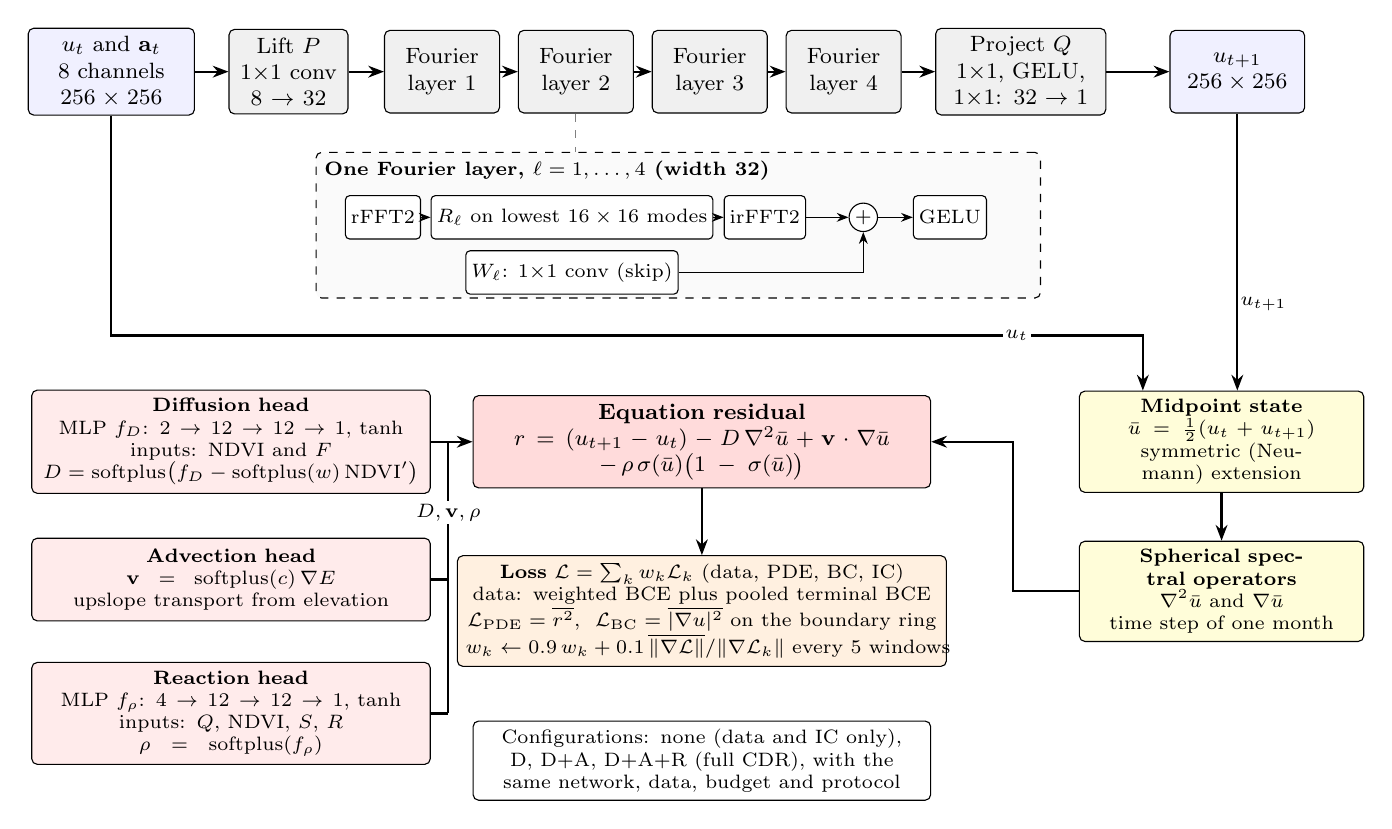
\begin{tikzpicture}[
  font=\footnotesize,
  blk/.style={draw, rounded corners=2pt, align=center, minimum height=1.05cm, fill=white, inner sep=3pt},
  inp/.style={blk, fill=blue!6},
  fno/.style={blk, fill=gray!12},
  head/.style={blk, fill=red!8, text width=4.85cm, font=\scriptsize},
  op/.style={blk, fill=yellow!15, text width=3.4cm, font=\scriptsize},
  los/.style={blk, fill=orange!12, text width=6.0cm, font=\scriptsize},
  sm/.style={draw, rounded corners=1.5pt, fill=white, font=\scriptsize, minimum height=0.55cm, inner sep=2pt, align=center},
  arr/.style={-{Stealth[length=2mm]}, thick},
  sarr/.style={-{Stealth[length=1.5mm]}}]
% ---------------- operator path (top row) ----------------
\node[inp, text width=1.9cm] (in)   at (1.10,0) {$u_t$ and $\mathbf{a}_t$\\8 channels\\$256\times256$};
\node[fno, text width=1.3cm] (lift) at (3.35,0) {Lift $P$\\1$\times$1 conv\\$8\to32$};
\node[fno, text width=1.25cm] (f1)  at (5.30,0) {Fourier\\layer 1};
\node[fno, text width=1.25cm] (f2)  at (7.00,0) {Fourier\\layer 2};
\node[fno, text width=1.25cm] (f3)  at (8.70,0) {Fourier\\layer 3};
\node[fno, text width=1.25cm] (f4)  at (10.40,0) {Fourier\\layer 4};
\node[fno, text width=1.95cm] (proj) at (12.65,0) {Project $Q$\\1$\times$1, GELU,\\1$\times$1: $32\to1$};
\node[inp, text width=1.5cm] (out)  at (15.40,0) {$u_{t+1}$\\$256\times256$};
\draw[arr] (in) -- (lift);
\draw[arr] (lift) -- (f1);
\draw[arr] (f1) -- (f2);
\draw[arr] (f2) -- (f3);
\draw[arr] (f3) -- (f4);
\draw[arr] (f4) -- (proj);
\draw[arr] (proj) -- (out);
% ---------------- inset: one Fourier layer ----------------
\node[draw, dashed, rounded corners=2pt, fill=gray!4, minimum width=9.2cm, minimum height=1.85cm] (inset) at (8.30,-1.95) {};
\node[anchor=north west, font=\scriptsize\bfseries, inner sep=3pt] at (inset.north west) {One Fourier layer, $\ell=1,\dots,4$ (width 32)};
\node[sm] (fft)  at (4.55,-1.85) {rFFT2};
\node[sm] (rw)   at (6.95,-1.85) {$R_\ell$ on lowest $16\times16$ modes};
\node[sm] (ifft) at (9.40,-1.85) {irFFT2};
\node[circle, draw, fill=white, inner sep=0.8pt, font=\scriptsize] (plus) at (10.65,-1.85) {$+$};
\node[sm] (gelu) at (11.75,-1.85) {GELU};
\node[sm] (skip) at (6.95,-2.55) {$W_\ell$: 1$\times$1 conv (skip)};
\draw[sarr] (fft) -- (rw);
\draw[sarr] (rw) -- (ifft);
\draw[sarr] (ifft) -- (plus);
\draw[sarr] (skip.east) -| (plus.south);
\draw[sarr] (plus) -- (gelu);
\draw[dashed, gray] (f2.south) -- (f2.south |- inset.north);
% ---------------- physics heads (left column) ----------------
\node[head] (hD) at (2.62,-4.70) {\textbf{Diffusion head}\\MLP $f_D$: $2\to12\to12\to1$, tanh\\inputs: NDVI and $F$\\\mbox{$D=\operatorname{softplus}\bigl(f_D-\operatorname{softplus}(w)\,\mathrm{NDVI}'\bigr)$}};
\node[head] (hv) at (2.62,-6.45) {\textbf{Advection head}\\$\mathbf{v}=\operatorname{softplus}(c)\,\nabla E$\\upslope transport from elevation};
\node[head] (hr) at (2.62,-8.15) {\textbf{Reaction head}\\MLP $f_\rho$: $4\to12\to12\to1$, tanh\\inputs: $Q$, NDVI, $S$, $R$\\$\rho=\operatorname{softplus}(f_\rho)$};
% ---------------- residual and loss (middle column) ----------------
\node[blk, fill=red!14, text width=5.6cm] (res) at (8.60,-4.70) {\textbf{Equation residual}\\$r=(u_{t+1}-u_t)-D\,\nabla^2\bar u+\mathbf{v}\cdot\nabla\bar u$\\$-\,\rho\,\sigma(\bar u)\bigl(1-\sigma(\bar u)\bigr)$};
\node[los] (loss) at (8.60,-6.85) {\textbf{Loss} \mbox{$\mathcal{L}=\sum_k w_k\mathcal{L}_k$} (data, PDE, BC, IC)\\
data: weighted BCE plus pooled terminal BCE\\
\mbox{$\mathcal{L}_{\mathrm{PDE}}=\overline{r^2}$,\ \ $\mathcal{L}_{\mathrm{BC}}=\overline{|\nabla u|^2}$ on the boundary ring}\\
\mbox{$w_k\leftarrow0.9\,w_k+0.1\,\overline{\|\nabla\mathcal{L}\|}/\|\nabla\mathcal{L}_k\|$ every 5 windows}};
\node[blk, fill=white, text width=5.6cm, minimum height=0.8cm, font=\scriptsize] (cfg) at (8.60,-8.75) {Configurations: none (data and IC only), D, D+A, D+A+R (full CDR), with the same network, data, budget and protocol};
% ---------------- derivatives (right column) ----------------
\node[op] (mid)  at (15.20,-4.70) {\textbf{Midpoint state}\\$\bar u=\tfrac12(u_t+u_{t+1})$\\symmetric (Neumann) extension};
\node[op] (spec) at (15.20,-6.60) {\textbf{Spherical spectral operators}\\$\nabla^2\bar u$ and $\nabla\bar u$\\time step of one month};
% ---------------- connections ----------------
\draw[arr] (in.south) -- (1.10,-3.35) -- (14.20,-3.35) -- (14.20,-3.35 |- mid.north);
\draw[arr] (out.south) -- (15.40,0 |- mid.north);
\node[font=\scriptsize, fill=white, inner sep=1pt] at (12.60,-3.35) {$u_t$};
\node[font=\scriptsize, fill=white, inner sep=1pt, right] at (15.40,-2.95) {$u_{t+1}$};
\draw[arr] (mid) -- (spec);
\draw[arr] (spec.west) -- (12.55,-6.60) -- (12.55,-4.70) -- (res.east);
\draw[thick] (hD.east) -- (5.38,-4.70);
\draw[thick] (hv.east) -- (5.38,-6.45);
\draw[thick] (hr.east) -- (5.38,-8.15);
\draw[thick] (5.38,-8.15) -- (5.38,-4.70);
\draw[arr] (5.38,-4.70) -- (res.west);
\node[font=\scriptsize, fill=white, inner sep=1pt] at (5.38,-5.60) {$D,\mathbf{v},\rho$};
\draw[arr] (res) -- (loss);
\end{tikzpicture}
\caption{Architecture of the CDR physics-informed neural operator. Top: the Fourier neural operator maps the state $u_t$ and seven covariates of month $t$ to $u_{t+1}$, with the structure of one Fourier layer shown in the inset. Bottom: three coefficient heads produce $D$, $\mathbf{v}$ and $\rho$, spherical spectral derivatives are evaluated on the midpoint state, and the equation residual enters the loss together with the data, boundary and initial terms under adaptive weights. The initial condition $u_0=0$ is imposed exactly, so $\mathcal{L}_{\mathrm{IC}}$ is identically zero. The four physics configurations differ only in which terms enter the residual.}
\label{fig:arch}
\end{figure*}

\subsubsection{Losses and training}
The residual of (\ref{eq:cdr}) is evaluated with a one-month forward difference and with spatial derivatives of the midpoint state $\bar u=(u_t+u_{t+1})/2$, computed by spherical spectral operators on a symmetric extension of the grid:
\begin{equation}
r=(u_{t+1}-u_t)-D\,\nabla^{2}\bar u+\mathbf{v}\cdot\nabla\bar u-\rho\,\sigma(\bar u)\bigl(1-\sigma(\bar u)\bigr).
\label{eq:residual}
\end{equation}
The data loss is a class-weighted binary cross entropy over all training cells, mixed in equal parts with a cross entropy on a log-sum-exp pooled terminal state for the final window. The boundary loss penalises $|\nabla u|^{2}$ on the boundary ring as a proxy for zero normal flux. Loss weights are updated every five windows by $w_k\leftarrow0.9\,w_k+0.1\,\overline{\|\nabla\mathcal{L}\|}/\|\nabla\mathcal{L}_k\|$, following the gradient balancing idea of \cite{wang2021gradient}. Training uses truncated backpropagation over windows of 24 months. Algorithm~\ref{alg:train} summarises one training epoch.

\begin{algorithm}[!t]
\caption{One training epoch of the operator}
\label{alg:train}
\small
\KwIn{monthly covariates $\mathbf{a}_{1:T}$, monthly fire indicators $y_{1:T}$, training mask $M$, configuration $\kappa\in\{\text{none},\text{D},\text{D+A},\text{D+A+R}\}$}
$u_0\leftarrow 0$\;
\For{each window $[t_0,t_0+23]$ of 24 months}{
  detach $u_{t_0}$ from the previous graph\;
  \For{$t=t_0$ \KwTo $t_0+23$}{
    $u_{t+1}\leftarrow\mathcal{G}_\theta(u_t,\mathbf{a}_t)$\;
    accumulate $\mathcal{L}_{\mathrm{data}}$ on cells in $M$\;
    \If{$\kappa\neq$ none}{compute $D,\mathbf{v},\rho$ from the heads; accumulate $\overline{r^2}$ using the terms enabled by $\kappa$; accumulate $\mathcal{L}_{\mathrm{BC}}$\;}
  }
  add pooled terminal cross entropy on the last state\;
  $\mathcal{L}\leftarrow\sum_k w_k\mathcal{L}_k$; update $\theta$ with AdamW\;
  every 5 windows update $w_k$ by gradient norm balancing\;
}
every 5 epochs compute validation \auc{}; reduce the learning rate on a plateau of validation loss; stop after 4 checks without improvement and restore the best checkpoint\;
\end{algorithm}

\subsection{Controlled Evaluation Design}
\subsubsection{Physics configurations}
Four configurations share the network, the data, the budget and the protocol: no physics (data and initial condition losses only), diffusion only, diffusion and advection, and the full equation.

\subsubsection{Evaluation tracks}
The tracks are listed in Table~\ref{tab:tracks}. For the held-out year track, the terminal label used in training is rebuilt from the training months only, since pooling it over all years would expose the test period.

\begin{table}[!t]
\caption{Evaluation Tracks Used for All Models}
\label{tab:tracks}
\centering
\footnotesize
\renewcommand{\arraystretch}{1.15}
\begin{tabular}{@{}lp{1.6cm}p{4.6cm}@{}}
\toprule
Track & Held-out unit & Construction \\
\midrule
A & random cells & 65/15/20 split of cells \\
B1 & spatial blocks & 2$^\circ\times$2$^\circ$ blocks in 3 folds; validation drawn as whole blocks from the training region \\
B2 & regions & 6 $k$-means regions, one held out at a time \\
B3 & years & test years 2000, 2008, 2009, 2015; validation years 2001, 2012, 2013, 2020; scored per cell and month \\
\bottomrule
\end{tabular}
\end{table}

\subsubsection{Protocol}
Every operator run used AdamW with a learning rate of $10^{-3}$ and a weight decay of zero (selected on validation), a learning rate reduced by half after two validation checks without improvement in validation loss, up to 80 epochs, and early stopping on validation \auc{} checked every five epochs with a patience of four checks. Seeds 42, 43 and 44 change only the initialisation and training noise; fold, region and year assignments are fixed. In total 102 runs were trained.

\subsubsection{Same-cell controls and baselines}
Random forest, MaxEnt and logistic regression were fitted on the operator's own 12 km cells, partitions and seven covariates. A second set used 12 km aggregates of the 55 predictors, which separates the effect of the predictors from that of the learner. For held-out years, two baselines ignore covariates: the fire frequency of each cell over the training years, and its frequency in the same calendar month. A random forest on the monthly covariates, with and without the month as an input, is also reported.

\subsubsection{Statistics}
Paired differences on identical test units were tested with the DeLong method \cite{delong1988} on tracks A and B3. On tracks B1 and B2, where test cells are clustered in space, a spatial block bootstrap with 123 blocks and 300 resamples was used. Calibration is summarised by the Brier score and the expected calibration error (ECE). Because non-forest cells can never be positive under a forest fire label, forest fraction alone reaches an \auc{} of 0.91 over all cells. Every classical result is therefore reported for all cells and for forest cells, with the forest population treated as primary, and each \auc{} is stated with its grid and prevalence.

\subsection{Physical Consistency Diagnostic}
For trained checkpoints (track A, seed 42, all configurations) we computed, over all valid cells and months, the median of $|\partial u/\partial t|$, the mean magnitude of each term on the right side of (\ref{eq:cdr}) and the root mean square of the residual (\ref{eq:residual}). A field that solves its equation should have a residual that is small relative to its own rate of change, and its rate of change should be clearly non-zero, because fire occurrence in India is strongly seasonal.

\subsection{Reimplementation of the Reference Protocol}
The protocol of \cite{biswas2025} was reimplemented on the present data with a 0.25$^\circ$ grid (4630 cells), the fifteen predictors as levels, presences from 2020 forest fires (1292 cells), MaxEnt with linear, quadratic, hinge and product features at a multiplier of one, and ten random 75/25 presence splits. The counts reported in \cite{biswas2025} (1830 training and 609 test presences) imply a 75/25 split, although the text states 70/30. This is a reimplementation and not the reference result.

%% =====================================================================
\section{Results}
\label{sec:results}
%% =====================================================================

\subsection{National Patterns}
Under Seasonal Kendall with false discovery rate control, NDVI increased significantly at 3\,552\,278 cells and decreased at 72\,305 (median Sen slope $+0.0026$ per year). Daytime land surface temperature decreased at 2\,435\,163 cells (median $-0.050\,^\circ$C per year), night-time temperature increased at 2\,080\,747 cells ($+0.024\,^\circ$C per year), and the diurnal range narrowed at 3\,273\,301 cells ($-0.077\,^\circ$C per year). Specific humidity increased at 26\,373 of 29\,056 climate cells, and air temperature changed significantly at 9\,988 cells, 7\,620 of them decreasing. The Mann-Kendall test applied to seasonal series had described the air temperature trend as noise, which the Seasonal Kendall result does not support. Global Moran's $I$ of NDVI over cells inside India is 0.9456 ($z=494$, $p=0.001$). Fire points lie on steeper terrain than the country as a whole (mean slope 12.35$^\circ$ against 5.72$^\circ$) and are 38.9\% closer to roads and 64.4\% closer to waterways than the national mean.

\subsection{Classical Models at 1 km}
Table~\ref{tab:classical} lists the classical results. Moving from all cells to forest cells lowers \auc{} by 0.08 to 0.15 and sharpens the ranking of learners. The random forest leads MaxEnt by 0.008 over all cells and by 0.031 over forest cells (paired DeLong). Spatial and regional hold-out lower forest \auc{} to 0.838 and 0.782. MaxEnt is better calibrated than the random forest (ECE 0.015 and 0.054 against 0.064 and 0.219 for all and forest cells), so the random forest output is interpreted as a relative score rather than a probability.

\begin{table}[!t]
\caption{Classical Models on the 1 km Test Set (All Cells / Forest Cells)}
\label{tab:classical}
\centering
\footnotesize
\renewcommand{\arraystretch}{1.15}
\begin{tabular}{@{}p{3.3cm}cc@{}}
\toprule
Model and track & \auc{} & Average precision \\
\midrule
RF, 55 features, A & \textbf{0.975 / 0.897} & 0.720 / 0.721 \\
MaxEnt, 55 features, A & 0.967 / 0.866 & 0.663 / 0.664 \\
RF, reference 15 predictors, A & 0.970 / 0.885 & 0.692 / 0.698 \\
RF, 55 features, B1 & 0.959 / 0.838 & 0.582 / 0.583 \\
MaxEnt, 55 features, B1 & 0.956 / 0.828 & 0.561 / 0.563 \\
RF, 55 features, B2 & 0.935 / 0.782 & 0.412 / 0.413 \\
RF, 55 features, B3 & 0.965 / 0.872 & 0.282 / 0.282 \\
Persistence baseline, B3 & 0.807 / 0.744 & 0.131 / 0.146 \\
\bottomrule
\multicolumn{3}{@{}p{8.4cm}@{}}{\scriptsize Prevalence 6.45\% (all) and 22.4\% (forest). Standard deviations over folds: B1 0.014 / 0.039 (RF), 0.012 / 0.029 (MaxEnt); B2 0.036 / 0.034 (RF).}
\end{tabular}
\end{table}

\subsection{RQ1: Physics Terms Against the Same Network Without Them}
Table~\ref{tab:ablation} and Fig.~\ref{fig:ablation} report the ablation. No configuration outperforms the network without physics on any track. Where the difference can be resolved (tracks A and B3), the physics terms lower the score, by 0.005 to 0.007 on track A (DeLong $p<0.02$ in each seed) and by 0.009 to 0.014 on track B3. On tracks B1 and B2 the block bootstrap intervals include zero. Diffusion alone is the weakest configuration wherever it was trained, and adding advection recovers most of the loss. The same ordering holds on forest cells (track A: 0.910 without physics against 0.897 with the full equation; track B3: 0.848 against 0.833). The physics terms increase training time by a factor of 2.3 to 2.4. Rebuilding the earlier held-out-year label, which included test years, changes the score by only 0.0006.

\begin{table}[!t]
\caption{Operator Ablation, Mean $\pm$ SD over Seeds and Folds (12 km Cells)}
\label{tab:ablation}
\centering
\footnotesize
\setlength{\tabcolsep}{3.2pt}
\renewcommand{\arraystretch}{1.15}
\resizebox{\columnwidth}{!}{%
\begin{tabular}{@{}lcccc@{}}
\toprule
Track & None & D & D+A & D+A+R \\
\midrule
A & \textbf{0.945}$\pm$0.002 & 0.924$\pm$0.005 & 0.939$\pm$0.001 & 0.939$\pm$0.002 \\
B1 & 0.724$\pm$0.010 & 0.642$\pm$0.013 & \textbf{0.730}$\pm$0.004 & 0.718$\pm$0.007 \\
B2 & \textbf{0.614}$\pm$0.021 & n/a & n/a & 0.570$\pm$0.007 \\
B3 & \textbf{0.904}$\pm$0.001 & 0.886$\pm$0.006 & 0.894$\pm$0.001 & 0.893$\pm$0.003 \\
\bottomrule
\end{tabular}}\\[3pt]
\parbox{\columnwidth}{\scriptsize D: diffusion, A: advection, R: reaction. Prevalence 42\% (A, cells) and 2.46\% (B3, cell-months). Full minus none, paired: A $-0.005$, $-0.007$, $-0.006$ (DeLong $p<0.02$ each seed); B1 and B2 intervals include zero; B3 $-0.010$, $-0.009$, $-0.014$.}
\end{table}

\begin{figure*}[!t]
\centering
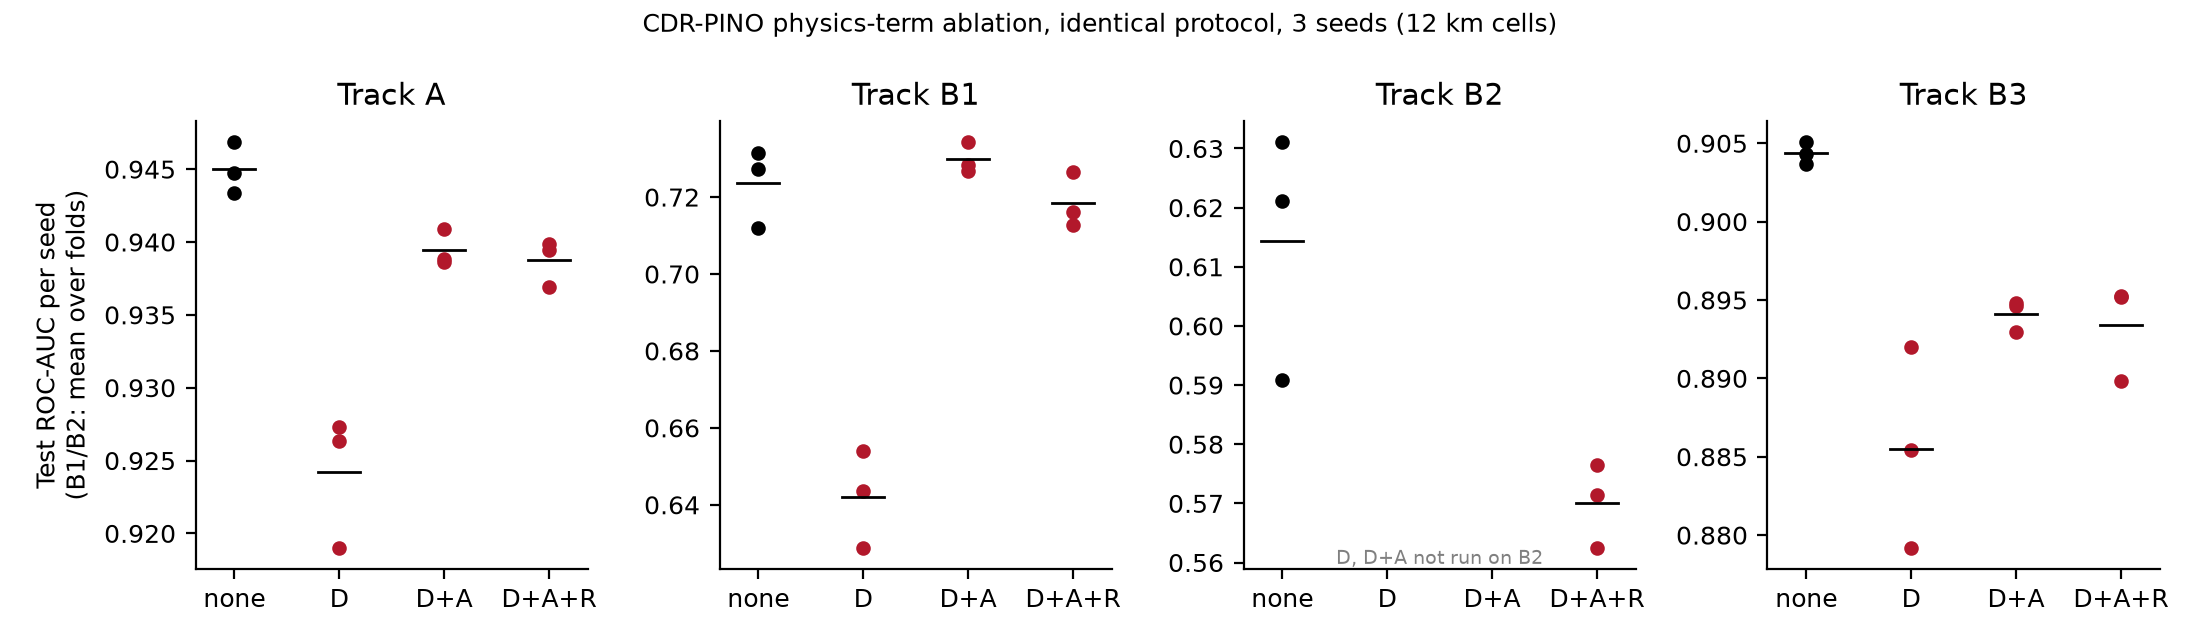
\includegraphics[width=\textwidth]{FigB_cdr_ablation_seeds.png}
\caption{Physics term ablation of the operator under an identical protocol. Dots are seeds (for B1 and B2, the mean over folds), horizontal lines are means. D, A and R denote diffusion, advection and reaction. Diffusion and diffusion with advection were not trained on track B2.}
\label{fig:ablation}
\end{figure*}

\subsection{RQ2: Classical Models on Identical Cells and Covariates}
Table~\ref{tab:samecells} and Fig.~\ref{fig:samecells} compare the operator with classical learners given the same cells, partitions and covariates. The random forest leads by 0.041 on track A, and the gap grows to 0.26 on B1 and 0.39 on B2. Even logistic regression on the same seven covariates exceeds the operator by 0.20 on B1 and 0.30 on B2. Replacing the seven covariates by 12 km aggregates of all 55 predictors changes the classical scores by at most 0.01 (random forest 0.981, 0.976 and 0.953), so the covariates are not what limits spatial transfer.

\begin{table}[!t]
\caption{Same 12 km Cells, Partitions and Covariates (All / Forest Cells)}
\label{tab:samecells}
\centering
\footnotesize
\setlength{\tabcolsep}{2.6pt}
\renewcommand{\arraystretch}{1.15}
\resizebox{\columnwidth}{!}{%
\begin{tabular}{@{}lccccc@{}}
\toprule
Track & CDR full & CDR none & LogReg & MaxEnt & RF \\
\midrule
A & 0.939/0.897 & 0.945/0.910 & 0.924/0.874 & 0.958/0.927 & \textbf{0.980/0.950} \\
B1 & 0.719/0.701 & 0.724/0.702 & 0.919/0.869 & 0.950/0.917 & \textbf{0.974/0.936} \\
B2 & 0.570/0.569 & 0.614/0.635 & 0.872/0.835 & 0.845/0.824 & \textbf{0.959/0.916} \\
\bottomrule
\end{tabular}}\\[3pt]
\parbox{\columnwidth}{\scriptsize B1 and B2 values are means over folds or regions.}
\end{table}

\begin{figure*}[!t]
\centering
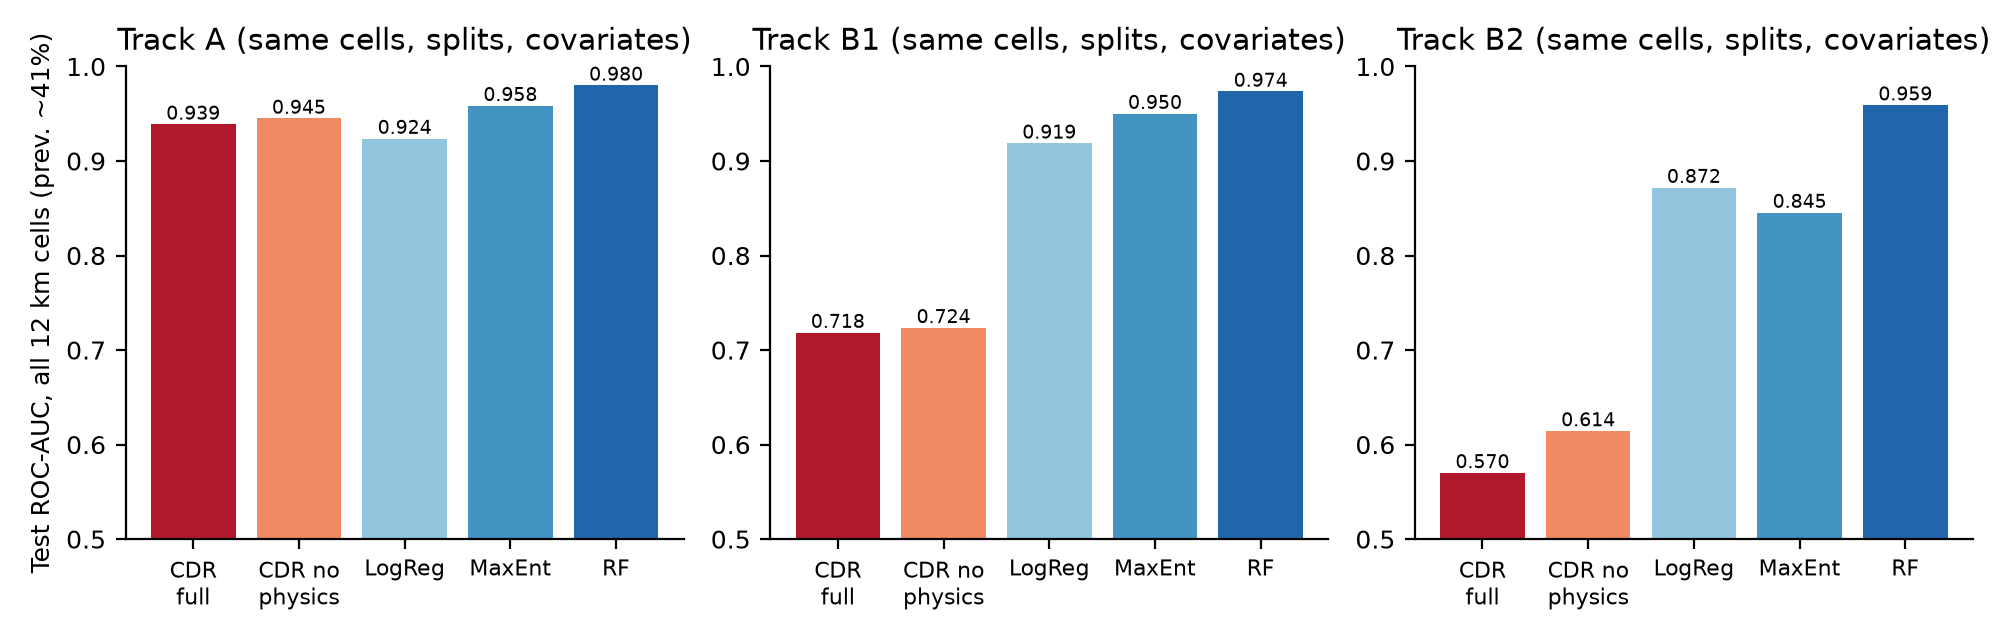
\includegraphics[width=\textwidth]{FigC_same_cells_cdr_vs_classical.png}
\caption{Test \auc{} of the operator and of classical learners fitted on the same 12 km cells, partitions and seven covariates, for random cells (A), spatial blocks (B1) and held-out regions (B2).}
\label{fig:samecells}
\end{figure*}

\subsection{RQ3: Held-Out Years Against Covariate-Free Baselines}
On the four held-out years, scored per cell and month at a prevalence of 2.46\%, the fire frequency of each cell over the training years reaches 0.908 (0.857 on forest cells), and the frequency in the same calendar month reaches 0.930 (0.920). The operator reaches 0.893 with the full equation and 0.904 without it. A random forest on the monthly covariates reaches 0.902, and 0.972 when the month is added (Fig.~\ref{fig:b3}). The operator's skill on unseen years is therefore below what the recurrence of fire at a location already provides. Most of the temporal signal is location combined with season, which a model given the calendar month captures directly.

\begin{figure}[!t]
\centering
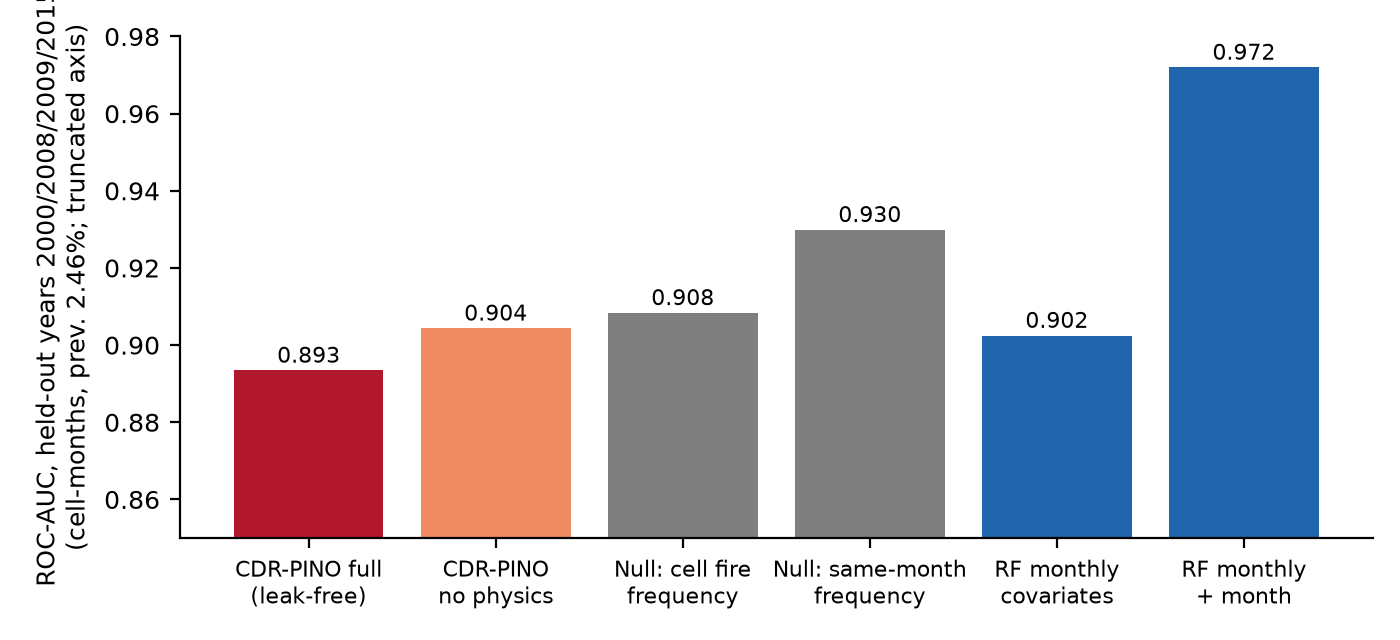
\includegraphics[width=\columnwidth]{FigD_B3_vs_nulls.png}
\caption{Held-out years (2000, 2008, 2009, 2015) scored per cell and month. The operator is compared with two covariate-free baselines and with random forests on monthly covariates.}
\label{fig:b3}
\end{figure}

\subsection{RQ4: Does the Trained Operator Solve Its Equation?}
\label{sec:rq4}
Table~\ref{tab:terms} and Fig.~\ref{fig:terms} summarise the term magnitudes. In every configuration the field is almost static, with a median $|\partial u/\partial t|$ of at most 0.002 per month despite the strong seasonality of fire. The root mean square residual is 74 to 616 times the mean rate of change, and diffusion contributes at most 0.3\% of the right side. The optimiser meets the data loss with a nearly static map and leaves the residual unresolved. Advection carries 83\% to 98\% of the right side, which indicates that the advective head mainly routes elevation information into the model. Within the seven-covariate model, removing elevation had the largest effect in an earlier single-seed jackknife test, which was not repeated here. With the full predictor set, however, the terrain group is redundant (Table~\ref{tab:decomp}). The prominence of elevation is therefore a property of the restricted covariate set rather than of fire occurrence.

\begin{table}[!t]
\caption{Term Magnitudes of Trained Track A Checkpoints (Seed 42)}
\label{tab:terms}
\centering
\footnotesize
\setlength{\tabcolsep}{3pt}
\renewcommand{\arraystretch}{1.15}
\begin{tabular}{@{}lccccc@{}}
\toprule
Config. & Median & \multicolumn{3}{c}{Share of right side} & Residual \\
\cmidrule(lr){3-5}
 & $|\partial_t u|$ & Adv. & React. & Diff. & ratio \\
\midrule
None & 0.0016 & 0.98 & 0.02 & 0.003 & 616 \\
D & 0.0003 & 0.83 & 0.16 & 0.002 & 224 \\
D+A & 0.0002 & 0.83 & 0.17 & 0.0004 & 74 \\
D+A+R & 0.0003 & 0.91 & 0.09 & 0.0004 & 78 \\
\bottomrule
\end{tabular}\\[3pt]
\parbox{\columnwidth}{\scriptsize Shares are fractions of the summed mean magnitudes of the three right-side terms, evaluated for every configuration with the full equation. Residual ratio: root mean square residual divided by the mean $|\partial_t u|$.}
\end{table}

\begin{figure}[!t]
\centering
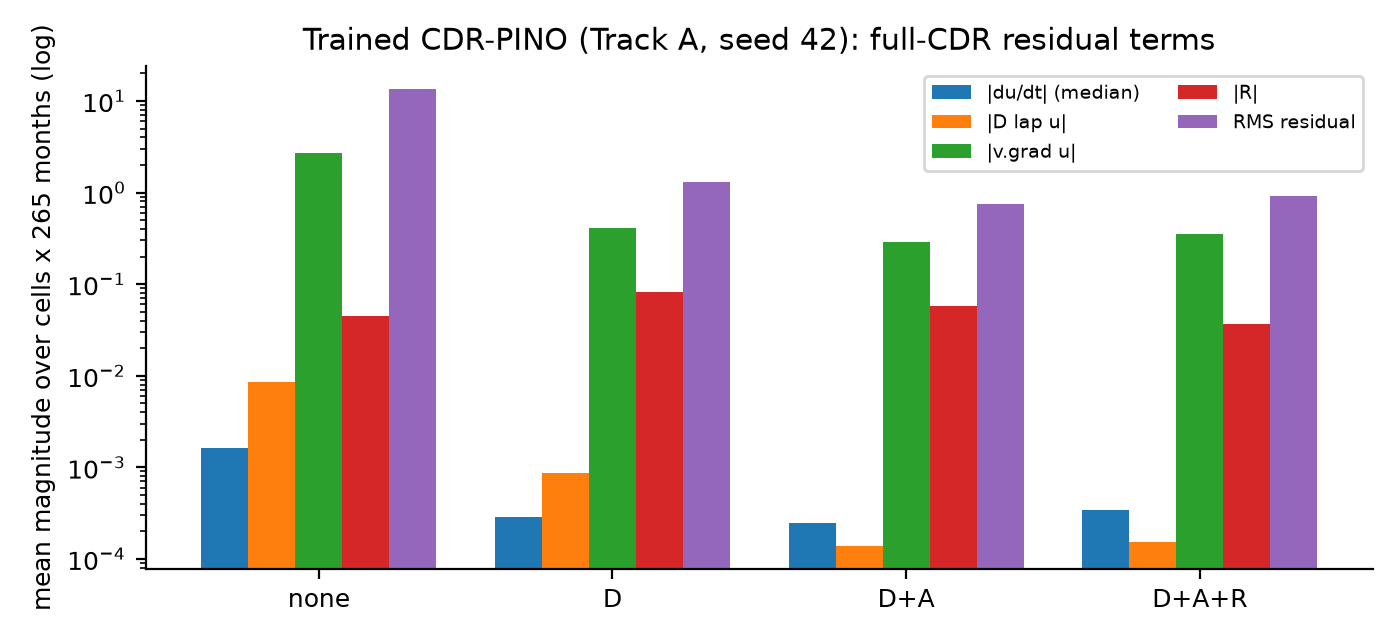
\includegraphics[width=\columnwidth]{FigG_cdr_term_magnitudes.png}
\caption{Mean magnitudes of the rate of change, of each right-side term and of the residual for trained track A checkpoints (log scale).}
\label{fig:terms}
\end{figure}

\subsection{Sources of the Accuracy Differences}
Table~\ref{tab:decomp} and Fig.~\ref{fig:decomp} decompose the differences with paired comparisons. The largest effects come from the model family and from the predictor set. Restricting the random forest to the operator's five static covariates costs 0.017 over all cells and 0.071 over forest cells. Trend and land cover groups add small but positive amounts, the terrain group is redundant, and neither the physics terms nor the operator structure contribute positively.

\begin{table}[!t]
\caption{Paired $\Delta$\auc{} Decomposition (All / Forest Cells)}
\label{tab:decomp}
\centering
\footnotesize
\renewcommand{\arraystretch}{1.15}
\begin{tabular}{@{}p{4.9cm}>{\raggedright\arraybackslash}p{3.3cm}@{}}
\toprule
Source of difference & $\Delta$\auc{} \\
\midrule
RF minus MaxEnt, reference 15 predictors & $+0.025$ / $+0.067$ \\
RF minus MaxEnt, 55 features & $+0.008$ / $+0.031$ \\
55 features minus reference 15 (RF) & $+0.005$ / $+0.012$ \\
55 features minus reference 15 (MaxEnt) & $+0.022$ / $+0.048$ \\
55 features minus operator's 5 static covariates (RF) & $+0.017$ / $+0.071$ \\
Trend group & $+0.001$ / $+0.006$ \\
Land cover group & $+0.003$ / $+0.008$ \\
Terrain group & $-0.0001$ / $-0.0006$ \\
Physics terms, full minus none (operator) & $-0.006$ (A), n.s. (B1, B2), $-0.011$ (B3) \\
Operator minus RF, same cells and covariates & $-0.041$ (A) \\
\bottomrule
\end{tabular}
\end{table}

\begin{figure*}[!t]
\centering
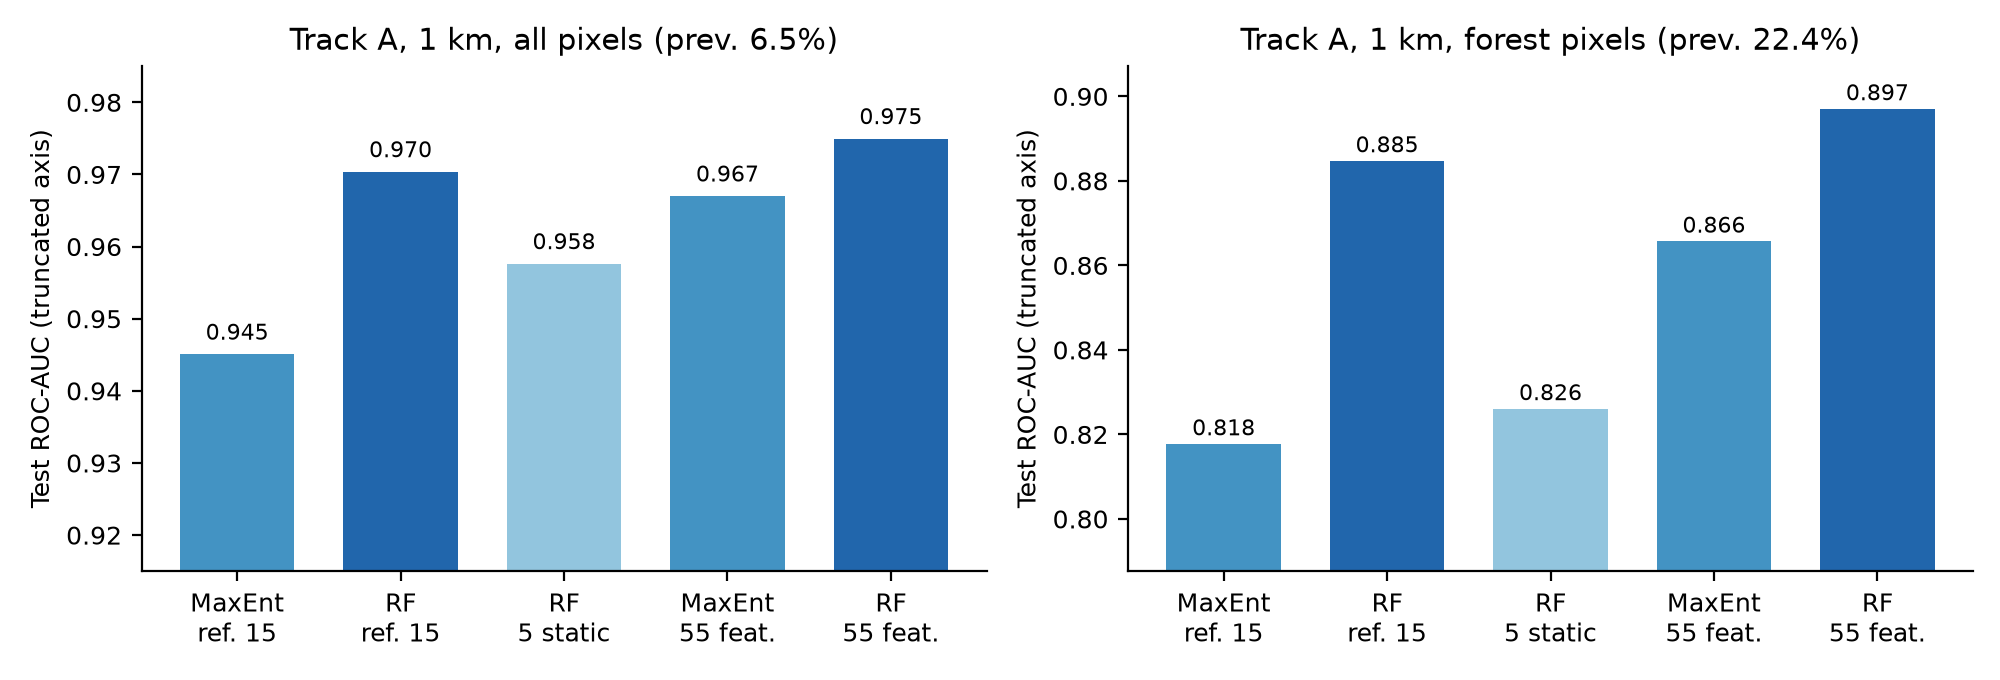
\includegraphics[width=0.82\textwidth]{FigA_contribution_1km.png}
\caption{Track A test \auc{} at 1 km for MaxEnt and random forest with the reference fifteen predictors (ref. 15), the operator's five static covariates (5 static) and the full 55 features (55 feat.), over all cells (left, prevalence 6.5\%) and forest cells (right, prevalence 22.4\%). The vertical axes are truncated.}
\label{fig:decomp}
\end{figure*}

\subsection{Relation to the Reference Study}
The reimplementation of the reference protocol reaches a test \auc{} of 0.893 $\pm$ 0.009 (range 0.877 to 0.912; training 0.902 $\pm$ 0.003), close to the 0.879 test and 0.894 training values reported in \cite{biswas2025}. The leading permutation importances are reproduced: NDVI 19.0\% (22.3\% in the reference), night land surface temperature 14.3\% (10.1\%), air temperature 13.2\% (13.1\%), day land surface temperature 8.1\% (9.6\%) and slope 5.8\% (5.6\%). Specific humidity (3.1\% against 13.0\%) is not reproduced, and elevation is ranked higher here (10.7\% against 2.4\%) (Fig.~\ref{fig:biswasimp} in the Appendix). The group totals reported in the reference study (33.9\%, 26.1\%, 10.8\% and 9.7\%) are permutation importances, although they are labelled as contributions. The pixel-level scores in Table~\ref{tab:classical} cannot be compared with the reference value, because the population, resolution, label and evaluation design all differ.

\subsection{National Susceptibility Map}
Fig.~\ref{fig:map} shows the track A random forest score at 1/120 degree, grouped into five classes by quantile breaks over forest cells (0.043, 0.210, 0.582 and 0.893). The map is distributed as a relative score and is tagged accordingly, since its mean (0.135) exceeds the prevalence (0.065) and no calibrated uncertainty estimate was established. High classes concentrate in the northeast, the central Indian highlands, the Eastern Ghats and the Himalayan foothills.

\begin{figure}[!t]
\centering
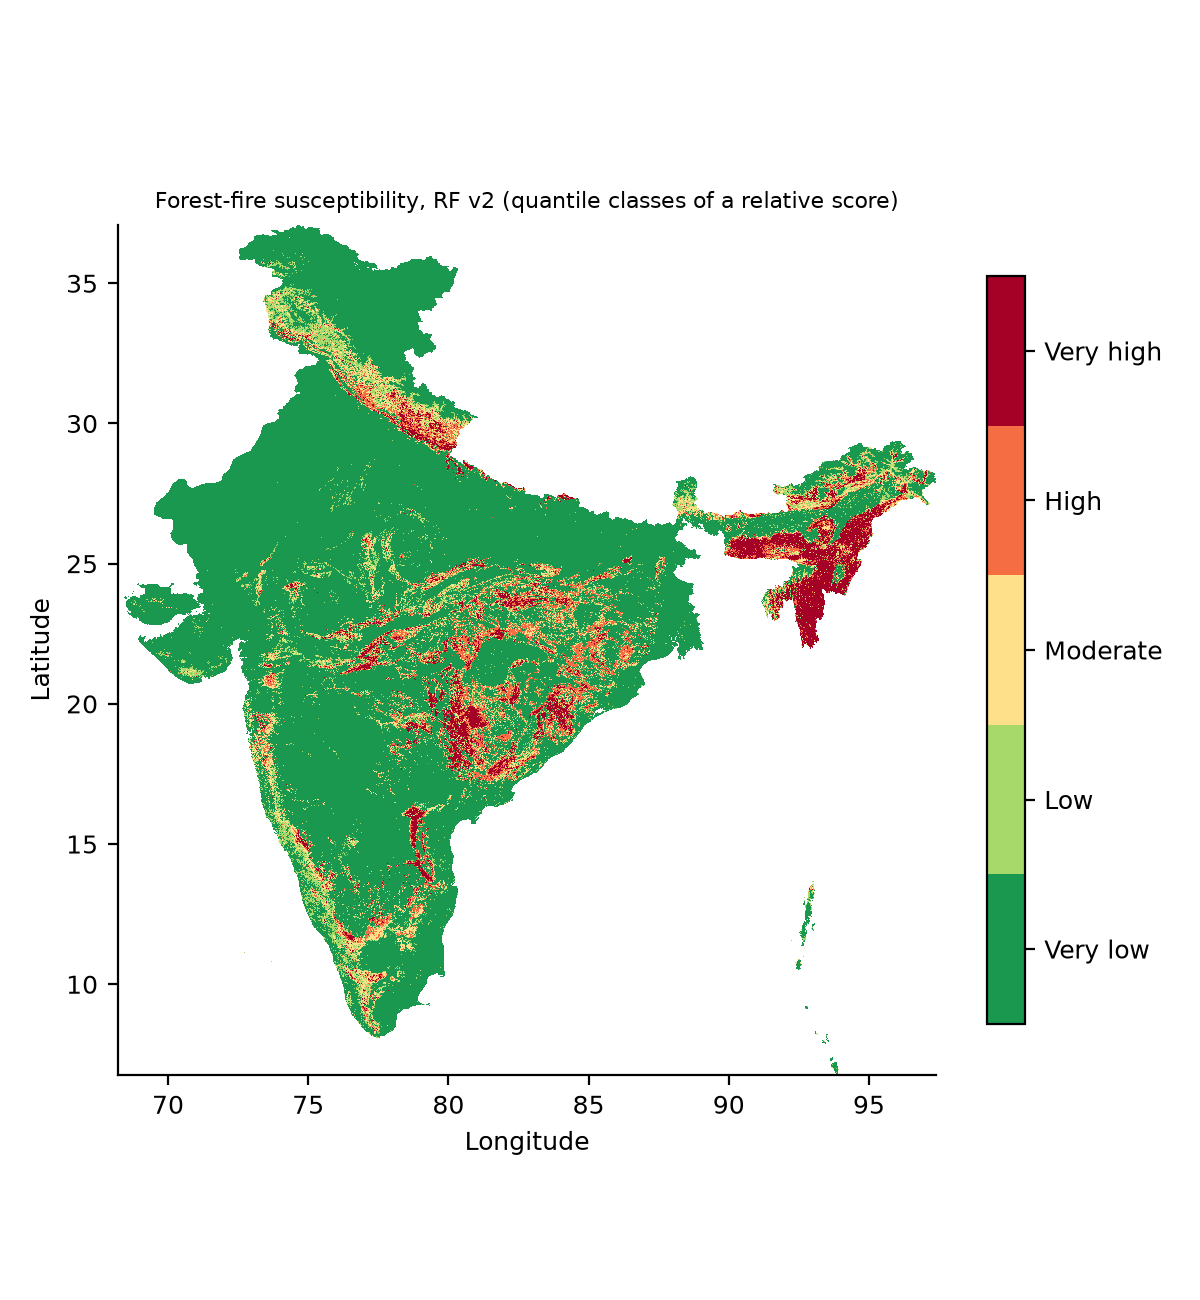
\includegraphics[width=\columnwidth]{FigH_final_map_RF_v2.png}
\caption{Forest fire susceptibility of India from the random forest with 55 features, shown as five quantile classes of a relative score computed over forest cells.}
\label{fig:map}
\end{figure}

%% =====================================================================
\section{Discussion}
\label{sec:discussion}
%% =====================================================================

\subsection{Why the Equation Did Not Help}
Four observations explain the negative result. First, the target is static while the equation is dynamic. Susceptibility, as defined here and in the reference study, is a long-run property of a place, so the data loss rewards a stable ranking of cells and the simplest optimum is a nearly static field, which is what the trained models produce. For a static field the right side of (\ref{eq:cdr}) would have to vanish, and nothing in the data enforces this, so the residual is absorbed rather than reduced. Second, the terms describe spread, whereas monthly detections aggregated to 12 km record where fires occur, not how they move between cells within a month. The negligible share of diffusion is consistent with this. Third, advection behaves as a channel for elevation: it carries most of the right side in every configuration and recovers most of what diffusion alone loses, yet terrain adds nothing once the full predictor set is available. Fourth, the weak spatial transfer belongs to the operator and not to the inputs. With identical cells and covariates, even a linear model transfers far better across blocks and regions. A global Fourier representation trained on a single national domain may tie distant regions together and learn structure that does not carry over to unseen areas. The network without physics shares this weakness, so the physics terms neither cause nor cure it.

\subsection{Implications for Physics-Informed Hazard Mapping}
The design included the conditions under which physics-informed models are usually expected to help, namely spatial, regional and temporal shift, sparse positives and several seeds, and no benefit appeared. This does not rule out physics-informed learning for fire. Spread prediction, where the equation describes the observed process, is a different problem. For susceptibility applications, the results suggest four minimum reporting elements: the same network without the equation, classical models on identical cells and covariates, covariate-free persistence baselines for any temporal claim, and a consistency check of the trained field against its equation.

\subsection{Lessons from the Pipeline}
Several defects corrected here are generic. Rounding coordinates against a raster edge moved three quarters of the fire points by one cell. A time mean of anomalies over its own baseline is degenerate. The Mann-Kendall test applied to seasonal or smoothed series misstates significance counts by large factors: here the Seasonal Kendall test found 6.7 times (day) to 117 times (night) more significant cells for land surface temperature, and for air temperature it reversed the earlier conclusion. Reporting all-cell scores for a forest label inflates accuracy because non-forest cells are trivially negative. None of these corrections changed any model score by more than 0.012, so the conclusions above do not depend on them, but the descriptive statistics that relied on the earlier choices were not valid.

\subsection{Limitations}
Only one operator family and one equation were tested, so the results do not exclude local operators or equations fitted to spread data. The operator's loss weights, number of modes and window length were not tuned beyond weight decay and early stopping. A larger search could narrow, but is unlikely to reverse, a gap of 0.26 to 0.39 under spatial hold-out. The global receptive field lets the operator see the covariates of test cells, never their labels, and the dryness index is standardised over all months; both effects would favour the operator. The operator runs at 12 km and the classical models at 1 km, which is why every operator comparison is made on the operator's own cells. The label records detected fire rather than burned area or severity, although annual forest-masked burned area correlates with the annual fire counts ($r=0.93$). The random forest map is a relative score without calibrated uncertainty. Resolution independence and fine-tuning of the operator were not evaluated and are not claimed. SHAP values could not be computed in the software environment used, so permutation importance and partial dependence were used instead.

%% =====================================================================
\section{Conclusion}
\label{sec:conclusion}
%% =====================================================================
We tested whether a convection-diffusion-reaction equation embedded in a neural operator improves forest fire susceptibility mapping over India, holding the architecture, inputs, grid and evaluation split fixed. The physics terms did not improve discrimination on any of four tracks and reduced it where the difference could be resolved. Classical learners on identical inputs outperformed the operator on every track, by 0.04 on random splits and by 0.26 to 0.39 under spatial and regional hold-out. On unseen years the operator fell below covariate-free persistence baselines, and the trained field was nearly static and did not satisfy its equation. The strongest model in this study is a random forest on a corrected set of 55 predictors, with a forest-cell \auc{} of 0.897 on a random split and 0.838 under spatial hold-out, and its advantage comes from the learner and the predictors. We recommend the controlled design and the consistency diagnostic as minimum practice for physics-informed hazard models, and release the corrected national pipeline, the reimplementation of the reference protocol (0.893 $\pm$ 0.009 against a reported 0.879), all per-cell predictions and all scripts.

%% =====================================================================
\section*{Data Availability}
The raw products are public (NASA FIRMS and LP DAAC, NASA GES DISC, ESA CCI and C3S, USGS SRTM and Geofabrik OpenStreetMap). The processing code for every step, the classical experiments, the operator training code (102 runs), the per-cell predictions, the analysis tables and the figures are available in the project repositories: \url{https://github.com/rawan230/Spatial_Mapping_INDIA-2000-2022-_}, \url{https://github.com/rawan230/Integrated-Fire-Risk-Analysis-in-India-and-Impliment-Baseline-Random-Forest-Model-} and \url{https://github.com/rawan230/_PINO_For_Spatial_Mapping_INDIA-2000-2022-}, together with the linked step repositories.

\section*{Acknowledgment}
The authors thank the providers of the MODIS, FLDAS, ESA CCI and C3S, SRTM and OpenStreetMap data.

%% =====================================================================
\appendices
\section{Supplementary Results}
\label{app:supp}
This appendix reports the permutation importance of the reimplemented reference protocol (Fig.~\ref{fig:biswasimp}), the sensitivity of MaxEnt to the number of training rows (Fig.~\ref{fig:maxentsize}) and the remaining sensitivity analyses (Table~\ref{tab:sens}). All values are read from the result files released with this study.

\begin{figure}[!ht]
\centering
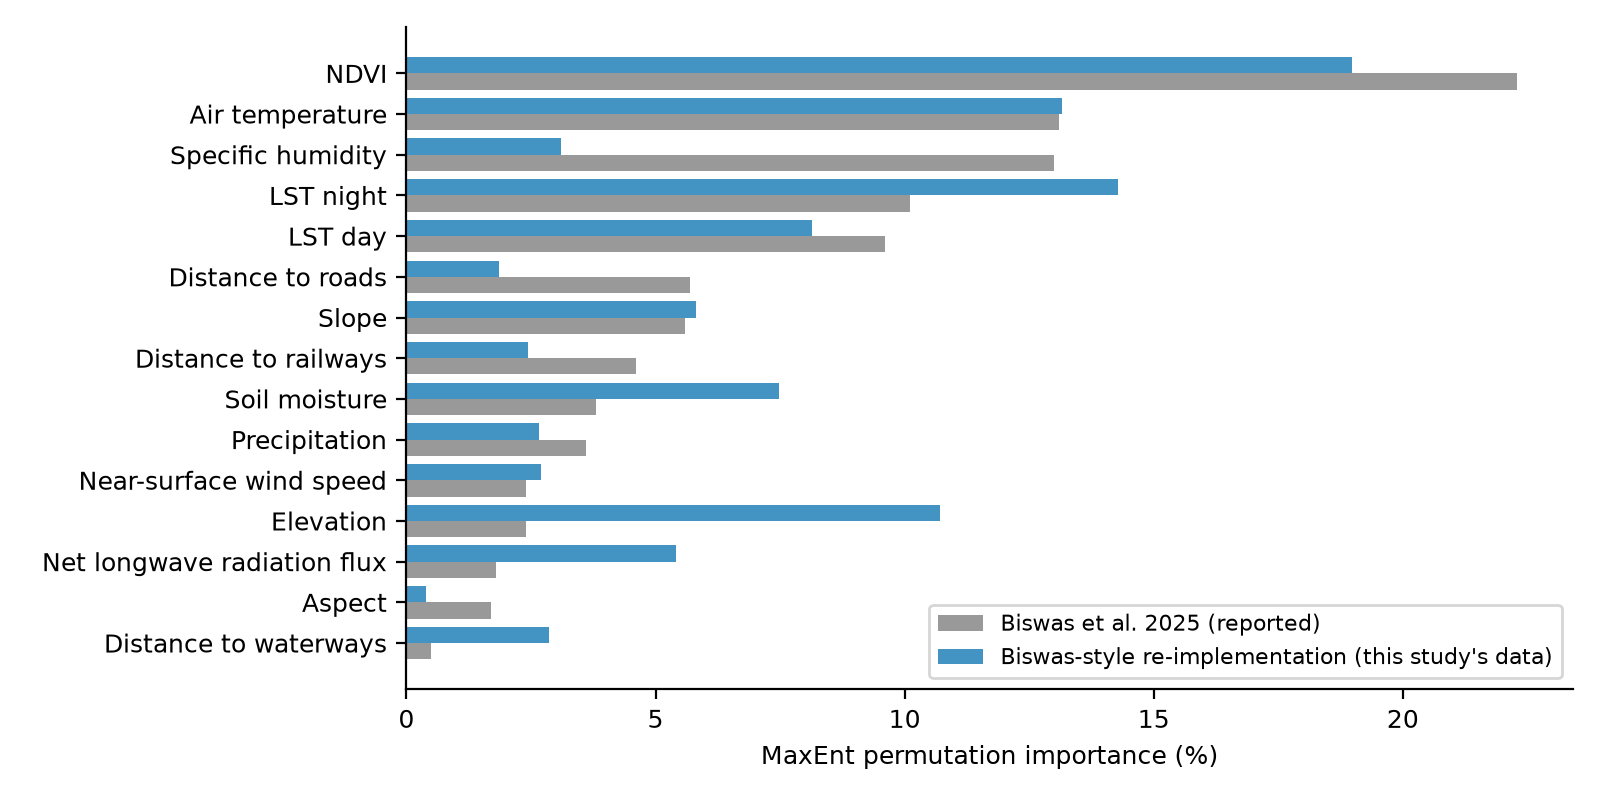
\includegraphics[width=\columnwidth]{FigF_biswas_importance_comparison.png}
\caption{Permutation importance of the reimplemented reference protocol compared with the values reported in \cite{biswas2025}.}
\label{fig:biswasimp}
\end{figure}

\begin{figure}[!ht]
\centering
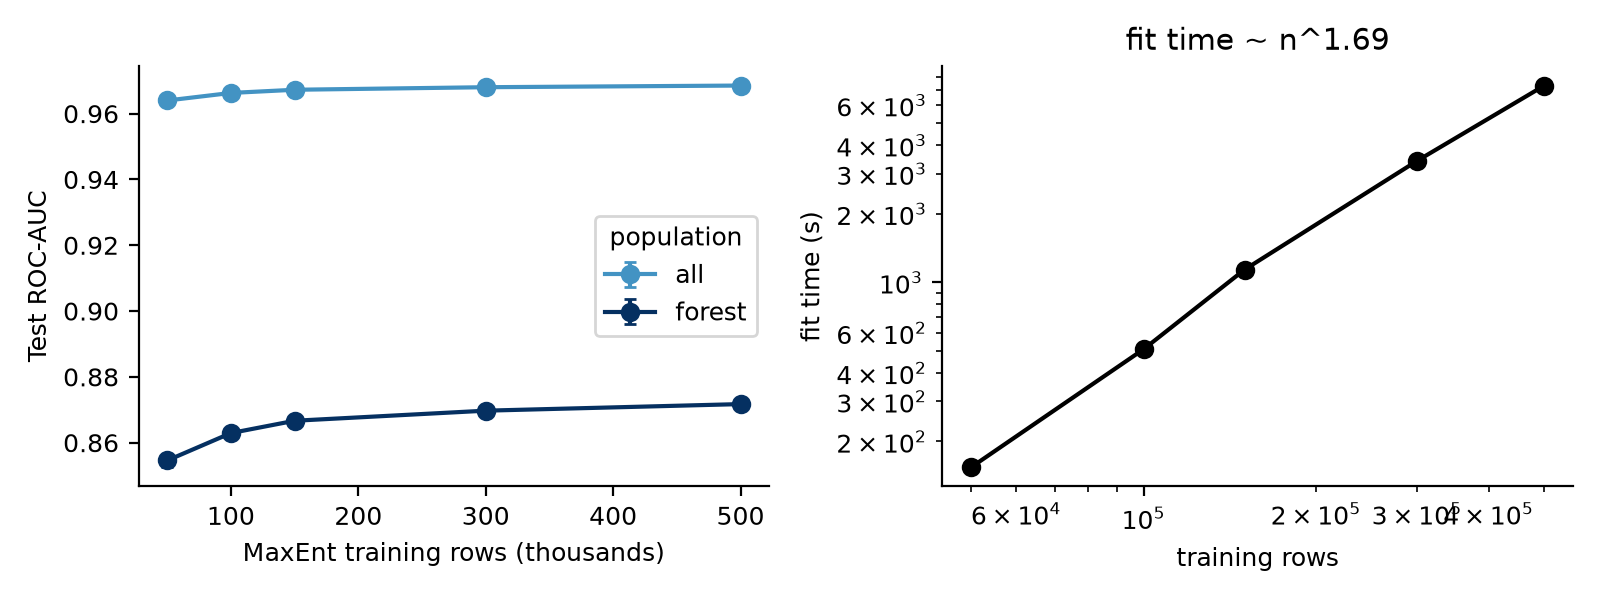
\includegraphics[width=\columnwidth]{FigE_maxent_sample_size.png}
\caption{MaxEnt test \auc{} and fitting time as a function of the number of training rows (50\,000 to 500\,000).}
\label{fig:maxentsize}
\end{figure}

\begin{table}[!ht]
\caption{Sensitivity Analyses (Random Forest, Track A Unless Stated)}
\label{tab:sens}
\centering
\footnotesize
\renewcommand{\arraystretch}{1.15}
\begin{tabular}{@{}p{4.6cm}p{3.4cm}@{}}
\toprule
Factor & Effect on \auc{} \\
\midrule
FIRMS confidence $\ge30$ and type 0 filters & $< 0.001$ \\
NDVI quality level (good only vs good and marginal) & negligible \\
LST aggregated to 0.05$^\circ$ (MOD11C3 resolution) & $\le 0.0002$ \\
Slope algorithm (Horn vs Zevenbergen-Thorne) & 0.0000 \\
Slope from a 0.25$^\circ$ DEM & negligible; mean slope 0.29$^\circ$ against 5.72$^\circ$ \\
Held-out year label built with test years (operator) & $+0.0006$ \\
MaxEnt rows 50k to 500k (all / forest) & 0.964 to 0.969 / 0.855 to 0.872; fit time grows as about $n^{1.6}$ \\
\bottomrule
\end{tabular}
\end{table}

\FloatBarrier
\bibliographystyle{IEEEtran}
\bibliography{references}

\end{document}
